% !TEX root = memoire.tex
\chapter{Enveloppe externe d'un chemin discret}\label{chapitre-chemins}

Nous présenterons dans ce chapitre un algorithme linéaire pour calculer l'enveloppe extérieure d'un chemin discret décrit par un code de Freeman. Le lien étroit entre un contour et un chemin simple mène à l'utilisation d'une structure d'arbre radix augmenté introduite par \cite{BKP} pour détecter les intersections, qui permet un stockage linéaire des points visités ainsi que leur liens de voisinage dans le plan discret $\Z \times \Z$. Cette structure de données combinée à l'algorithme de la main droite, bien connu pour la résolution de labyrinthe, permet d'obtenir un algorithme linéaire pour calculer l'enveloppe externe. Les résultats de ce chapitre ont été présentés à la conférence internationale DGCI 2014 \cite{BTTW14}.

\begin{figure}[H]
\centering
\includegraphics[width=0.8\textwidth]{fourmi}
\caption{L'algorithme glouton de la chenille produit un chemin simple.}
\end{figure}

\section{Les chemins}\label{chemins:preliminaires}


\begin{definition}
L'\emph{ensemble de pas unitaires} est l'ensemble des points de $\Z^2$ accessibles à partir de $(0,0)$ en une seule opération.
\end{definition}

Les pas élémentaires de l'alphabet de Freeman forment un ensemble de pas unitaire.
$$\mathcal{F}=\left\{0,1,2,3\right\} \simeq \left\{(1,0),(0,1),(−1,0),(0,−1)\right\}$$

\begin{definition}
Soit $P$ un ensemble de pas unitaires. Un \emph{chemin} $c=c_0,c_1,...,c_{n-1}$ est une suite de points tels que pour tout $i>0$, il existe au moins un $p\in P$ tel que $c_{i} = c_{i-1} + p$.
\end{definition}

On remarque que $c_0$ est indépendant de $P$. On peut ancrer un chemin n'importe où.

\begin{proposition}
Soit $P=\left\lbrace (1,0),(0,1),(-1,0),(0,-1) \right\rbrace$. Pour tout chemin $C$ à pas unitaires dans $P$ enraciné en $c_0 \in \Z^2$, on a $C \subset \Z^2$.
\end{proposition}
 
\begin{definition}
Un chemin est \emph{discret} lorsque tous ses points sonts dans $\Z^2$.
\end{definition}

On vérifie facilement que si $c_0$ est à coordonnées entières, un chemin est discret.
 
\begin{definition}
Un chemin est \emph{fermé} s'il existe un pas unitaire $p$ tel que $c_0 = c_{n-1}+p$.
\end{definition}

\begin{definition}
Un chemin est \emph{simple} si ses points sont visités exactement une fois. Un chemin simple peut être \emph{fermé} si seul son point d'origine est visité une deuxième fois, au dernier pas.
\end{definition}

Il y a une bijection entre les cellules et $\Z^2$ obtenue en associant $(a,b)\in \Z^2$ au carré unitaire dont le coin inférieur gauche est de coordonnée $(a,b)$. Ainsi, on peut considérer les cellules comme des éléments de $\Z^2$. Par définition, un \emph{ensemble discret} $S$ est un ensemble de cellules, i.e. $S\subset \Z^2$.

Une façon pratique de représenter un ensemble connexe discret sans trous est d'utiliser un mot décrivant son contour. Puisque le contour d'un ensemble discret est un chemin, on utilise le codage de Freeman qui représente efficacement un chemin discret dans $\Z^2$.

\newcommand{\firstdifference}{\ensuremath{\mathbf{\Delta}}}

Il est clair de ces définitions que tout chemin discret $C$ est représenté par un mot $w\in \F^*$ où $\F=\{\ocr{0},\ocr{1},\ocr{2},\ocr{3}\}$ est l'alphabet de Freeman. Il est intéressant de mentioner ici que dans le cas d'un chemin discret fermé, $w$ est unique à permutation circulaire des lettres près. On peut vérifier à l'aide de la figure \ref{fig:2.1} que toute permutation circulaire du mot $w=\ocr{001100322223}$ représente le même chemin, que $w$ est non simple, fermé, et que $$\firstdifference(w)=\ocr{01030330001}$$
code bien les virages de $w$.

\begin{figure}
\begin{subfigure}[b]{.5\textwidth}
\centering
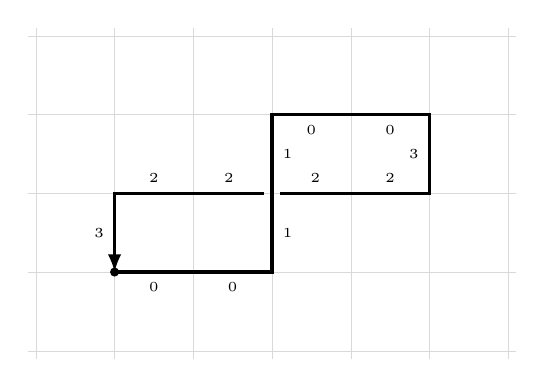
\begin{tikzpicture}[
	l/.style={font=\tiny}, >=latex, auto]
	\draw[help lines, opacity=0.3] (-0.1,-0.1) grid (6.1, 4.1);
	\node[circle, draw, fill, inner sep=1] at (1,1) {};

	\draw[very thick] (1,1) --node[l, swap]{0} ++(1,0)  --node[l, swap]{0} ++(1,0)  --node[l, swap]{1} ++(0,1)  --node[l, swap]{1} ++(0,1)  --node[l, swap]{0} ++(1,0)  --node[l, swap]{0} ++(1,0)  --node[l, swap]{3} ++(0,-1)  --node[l, swap]{2} ++(-1,0)  --node[l, swap]{2} ++(-0.9,0);
	\draw[very thick] (2.9,2)  --node[l,swap]{2} ++(-0.9,0)  --node[l,swap]{2} ++(-1,0) --node[l,swap]{3} ++(0,-1)[->];


\end{tikzpicture}
\caption{$w=\ocr{001100322223};$}\label{fig:2.1a}
\end{subfigure}
\begin{subfigure}[b]{.5\textwidth}
\centering
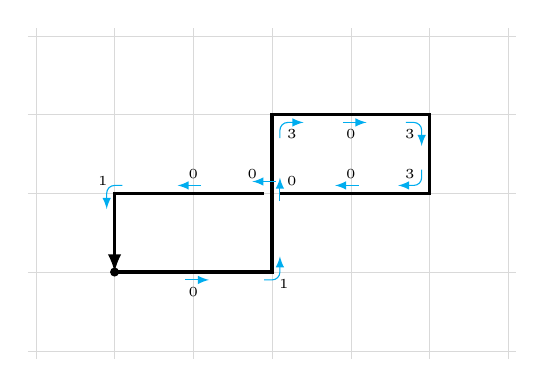
\begin{tikzpicture}[polyomino/.style={red, very thick, fill=red, fill opacity=0.3}, l/.style={font=\tiny}, >=latex]
	\draw[help lines, opacity=0.3] (-0.1,-0.1) grid (6.1, 4.1);
	%\draw[very thick,->] (0,0) -- (0, 4.3);
	%\draw[very thick,->] (0,0) -- (6.3, 0);
	\node[circle, draw, fill, inner sep=1] at (1,1) {};

	\draw[very thick] (1,1) --++(1,0)  --++(1,0)  --++(0,1)  --++(0,1)  --++(1,0)  --++(1,0)  --++(0,-1)  --++(-1,0)  --++(-0.9,0);
	\draw[very thick] (2.9,2)  --++(-0.9,0)  --++(-1,0) --++(0,-1)[->];

	\draw[cyan] (1.9,0.9) -- ++(0.3, 0)[->];
	\draw[cyan] (2.9,0.9) -- ++(0.1, 0) arc (-90:0:0.1) -- ++(0,0.2)[->];
	\draw[cyan] (3.1,1.9) -- ++(0, 0.3)[->];
	\draw[cyan] (3.1,2.7) -- ++(0, 0.1) arc (180:90:0.1) -- ++(0.2,0)[->];

	\draw[cyan] (3.9,2.9) -- ++(0.3, 0)[->];
	\draw[cyan] (4.7,2.9) -- ++(0.1, 0) arc (90:0:0.1) -- ++(0,-0.2)[->];
	\draw[cyan] (4.9,2.3) -- ++(0,-0.1) arc (0:-90:0.1) -- ++(-0.2,0)[->];
	\draw[cyan] (4.1,2.1) -- ++(-0.3,0)[->];
	\draw[cyan] (3.05,2.15) -- ++(-0.3,0)[->];
	\draw[cyan] (2.1,2.1) -- ++(-0.3,0)[->];
	\draw[cyan] (1.1,2.1) -- ++(-0.1,0) arc (90:180:0.1) -- ++(0,-0.2)[->];
	
	\node[l] at (2,0.75) {0};
	\node[l] at (3.15,0.85) {1};
	\node[l] at (3.25,2.15) {0};
	\node[l] at (3.25,2.75) {3};
	\node[l] at (4,2.75) {0};
	\node[l] at (4.75,2.75) {3};
	\node[l] at (4.75,2.25) {3};
	\node[l] at (4,2.25) {0};
	\node[l] at (2.75,2.25) {0};
	\node[l] at (2,2.25) {0};
	\node[l] at (0.85,2.15) {1};
\end{tikzpicture}
\caption{$\firstdifference(w)=\ocr{01030330001};$}\label{fig:2.1b}
\end{subfigure}
\caption{Deux codages du même chemin}\label{fig:2.1}
\end{figure}

Tout chemin est contenu dans un plus petit rectangle, appelé la \emph{boîte englobante} (ou \emph{bounding box} en anglais). On définit $W$ comme étant le point le plus bas parmi les points les plus à gauche sur cette boîte tel qu'illustré à la figure \ref{fig:point-W}. On peut facilement obtenir $W$ en temps linéaire en lisant le mot une première fois en conservant les extremums.


\begin{figure}
\begin{subfigure}[b]{.5\linewidth}
\centering
\shorthandoff{:}
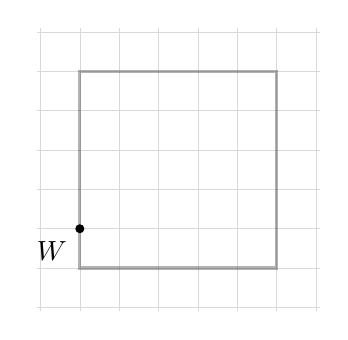
\begin{tikzpicture}[>=latex, scale=0.5]
	\draw[help lines, opacity=0.3] (-0.1,-0.1) grid (7.1, 7.1);
	\simplepath[->, very thick]{(3,6)}{6446660246000600224};
	\draw[very thick, opacity=0.3] (1,1) rectangle (6,6);
	\node[circle, draw, fill, inner sep=1, label=below left:{$W$}] at (1,2) {};
\end{tikzpicture}
\caption{}\label{fig:point-Wa}
\end{subfigure}
\begin{subfigure}[b]{.5\linewidth}
\centering
\shorthandoff{:}
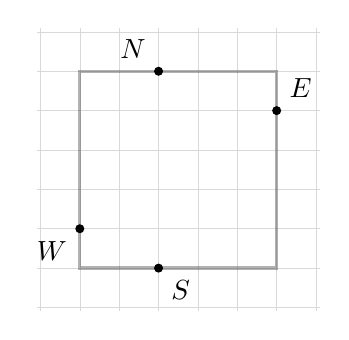
\begin{tikzpicture}[>=latex, scale=0.5]
	\squarepath{(1,2)}{06200244202060};
	\draw[help lines, opacity=0.3] (-0.1,-0.1) grid (7.1, 7.1);
	\draw[very thick, opacity=0.3] (1,1) rectangle (6,6);
	\node[circle, draw, fill, inner sep=1, label=below left:{$W$}] at (1,2) {};
	\node[circle, draw, fill, inner sep=1, label=below right:{$S$}] at (3,1) {};
	\node[circle, draw, fill, inner sep=1, label=above right:{$E$}] at (6,5) {};
	\node[circle, draw, fill, inner sep=1, label=above left:{$N$}] at (3,6) {};
\end{tikzpicture}
\caption{}\label{fig:point-Wb}
\end{subfigure}
\caption{Boîte englobante et factorisation standard}\label{fig:point-W}
\end{figure}

On termine cette section avec un bref rappel de topologie des graphes (voir \cite{gross87} pour un traitement plus complet du sujet). Soit $P$ un chemin discret (i.e. une suite de points entiers) codés par le mot $w$. L'image de $P$ comme un sous-ensemble de $\R^2$ est notée $G_P$ tandis que le graphe de l'image plongé dans le dans le plan $\R^2$ est notée $\mathcal{G}(P)$.

Le \emph{plongement} d'un graphe $G$ sur une surface $S$ fait correspondre des points de $S$ aux sommets de $G$ et des \emph{arcs simples} (images homéomorphiques de $[0,1]$) aux arêtes de $G$ de telle façon à ce que :

\begin{itemize}
\item Les extrémités de l'arc associé à l'arête $e$ sont les points associés aux sommets aux extrémités de $e$.
\item Aucun arc ne contient de points associés à un autre sommet.
\item Deux arcs ne se croisent pas en un point contenu dans l'un des deux arcs.
\end{itemize}

Intuitivement, cela signifie que les arcs ne se croisent pas et ne passent pas par un sommet.

Dans le cas du graphe associé au chemin discret $P$, un tel plongement est complètement déterminé en associant un ordre cyclique aux arêtes autour de chaque sommet de la façon suivante : d'abord on fixe une orientation en chaque point (par exemple anti-horaire). Ensuite, pour chaque sommet $v$ dans $G_P$, on définit la permutation cyclique sur les arêtes entrantes de $v$. Ceci définit un schéma de rotation sur $G_P$. On peut montrer qu'un tel schéma de rotation est équivalent à un plongement orienté de $G_P$ sur une surface. Par exemple, la figure \ref{fig:plongement} illustre le chemin $P$ codé par $w=\ocr{001322}$, son graphe $G_P$ et son plongement anti-horaire $\mathcal{G}_P$ dans $\R^2$.

\begin{figure}
\centering
\begin{subfigure}[b]{.3\linewidth}
\centering
\shorthandoff{:}
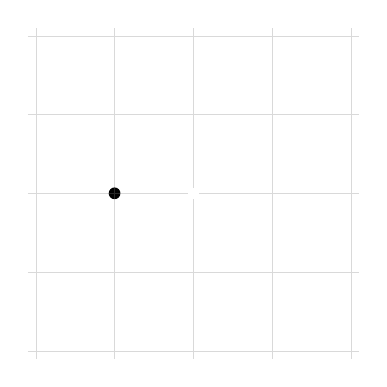
\begin{tikzpicture}[>=latex, scale=1]
	\node[fill, circle, inner sep=1.5] at (1,2) {};
	\draw[help lines, opacity=0.3] (-0.1,-0.1) grid (4.1, 4.1);
	\simplepath[->, very thick]{(2,2)}{02466};
	\node[fill=white, inner sep=0.2em] at (2,2) {};
	\simplepath[very thick]{(1,2)}{00};
\end{tikzpicture}
\caption{}
\end{subfigure}
\begin{subfigure}[b]{.3\linewidth}
\centering
\shorthandoff{:}
\begin{tikzpicture}[>=latex, scale=1,
	sommet/.style={fill, circle, inner sep=1.5}]
	\node[fill=white, inner sep=0.5em] at (2,2) {};
	\simplepath[very thick]{(1,2)}{002466};
	\node[sommet, label=west:{A}] at (1,2) {};
	\node[sommet, label=north west:{E}] at (2,2) {};
	\node[sommet, label=south east:{D}] at (3,2) {};
	\node[sommet, label=north east:{C}] at (3,3) {};
	\node[sommet, label=north west:{B}] at (2,3) {};
	\node[sommet, label=south:{F}] at (2,1) {};
\end{tikzpicture}
\caption{}
\end{subfigure}
\begin{subfigure}[b]{.3\linewidth}
\centering
\renewcommand{\arraystretch}{0.6}
\begin{tabular}{rcl}
A & : & E\\
B & : & C E\\
C & : & B D\\
D & : & C E\\
E & : & A F D B\\
F & : & E\\
\end{tabular}
\caption{}
\end{subfigure}
\caption{(a) Le graphe $G_P$ codé par le mot $w=\ocr{001233}$; (b) Le plongement anti-horaire de $\mathcal{G}(P)$ dans $\R^2$; (c) Le schéma de rotation de $\mathcal{G}(P)$.}\label{fig:plongement}
\end{figure}

Puisque par définition un plongement de $P$ est planaire, la surface sur laquelle $P$ est plongée se trouve partagée en un certain nombre de régions mutuellement exclusives délimitées par $\mathcal{G}(P)$. On nomme ces régions \emph{faces} et dans le cas d'une surface infinie comme $\R^2$, toutes les faces sont de taille finie sauf une. Cette face non-bornée est la \emph{face externe} de $\mathcal{G}(P)$.

\section{Enveloppes externes et convexes}

\newcommand{\hull}[1]{\text{Hull}(#1)}

On rappelle qu'en topologie, étant donné un ensemble $S$, le bord $\partial S$ est l'ensemble des points dans l'adhérence de $S$ qui ne sont pas à l'intérieur de $S$. L'\emph{enveloppe externe} de $S$, notée $\hull{S}$, est le bord de l'intersection de tous les ensembles discrets sans trous contenant $S$, i.e. le chemin simple suivant le contour de $S$. La définition \ref{def:outer-hull} étend la notion d'enveloppe externe à tout chemin discret.

\begin{definition}\label{def:outer-hull}
Soit $P$ un chemin discret. Alors, l'enveloppe externe de $P$, notée $\hull{P}$ est la face externe de $\mathcal{G}(P)$, le plongement de $P$.
\end{definition}

On note que la définition \ref{def:outer-hull} utilise le plongement de $P$ plutôt qu'un ensemble discret pour décrire l'enveloppe externe. Ce choix permet de décrire l'enveloppe d'un chemin discret (i.e. un ensemble Euclidien d'aire $0$). Par exemple, la figure \ref{chemin-et-enveloppe-externe} illustre l'enveloppe externe du chemin $w=021$.  On remarque aussi qu'en utilisant la définition \ref{def:outer-hull}, le bord d'un chemin est codé par un mot fermé. e.g. l'enveloppe externe du chemin codé par $0$ est codé par $02$. Ainsi, la définition \ref{def:outer-hull} offre une généralisation adéquate de l'enveloppe externe aux chemins discrets quelconques. En effet, si $P$ code le bord d'un ensemble discret sans trou $S$, alors $P$ est simple et fermé par définition. Donc $P=\hull{P}$ et donc puisque $\hull{S}$ est le bord $\partial S$ de $S$ par définition, on a
\begin{equation}
\hull{S} = \partial S = P = \hull{P}\text{.}
\end{equation}

\begin{figure}
\centering
\begin{subfigure}[b]{.3\textwidth}
\centering
\shorthandoff{:}
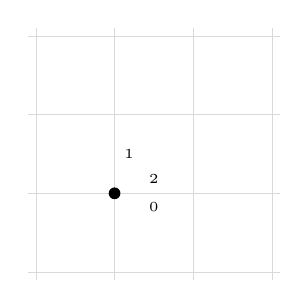
\begin{tikzpicture}[>=latex, scale=1, auto]
	\draw[help lines, opacity=0.3] (-0.1,-0.1) grid (3.1, 3.1);
	\node[fill, circle, inner sep=1.5] at (1,1) {};
	\simplepath[->, very thick]{(1,1)}{042};
	\path (1,1) -- node[swap]{\tiny 0} (2,1) -- node[swap]{\tiny 2} (1,1) -- node[swap]{\tiny 1} (1,2);
\end{tikzpicture}
\end{subfigure}
\begin{subfigure}[b]{.3\textwidth}
\centering
\shorthandoff{:}
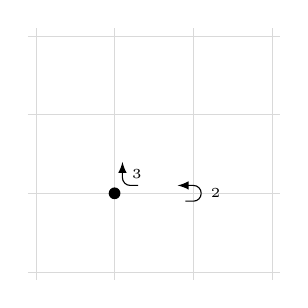
\begin{tikzpicture}[>=latex, scale=1, auto]
	\draw[help lines, opacity=0.3] (-0.1,-0.1) grid (3.1, 3.1);
	\node[fill, circle, inner sep=1.5] at (1,1) {};
	\simplepath[->, very thick]{(1,1)}{042};
	\draw[rounded corners=2.8pt, ->] (1.9, 0.9) -- (2.1, 0.9) -- node[swap, midway]{\tiny $2$} (2.1,1.1) -- (1.8, 1.1);
	\draw[rounded corners=2.8pt, ->] (1.3, 1.1) -- (1.1, 1.1) -- node[swap]{\tiny $3$} (1.1, 1.4);
\end{tikzpicture}
\end{subfigure}
\begin{subfigure}[b]{.3\textwidth}
\centering
\end{subfigure}
\begin{subfigure}[b]{.3\textwidth}
\centering
\shorthandoff{:}
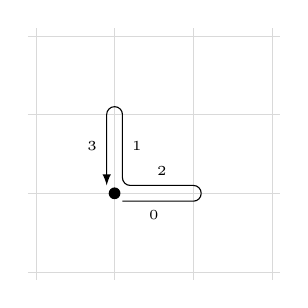
\begin{tikzpicture}[>=latex, scale=1, auto]
	\draw[help lines, opacity=0.3] (-0.1,-0.1) grid (3.1, 3.1);
	\node[fill, circle, inner sep=1.5] at (1,1) {};
	\simplepath[->, very thick]{(1,1)}{042};
	\draw[rounded corners=2.8pt, ->] (1.1, 0.9) --node[swap, midway]{\tiny $0$} (1.9, 0.9) -- (2.1, 0.9) -- (2.1,1.1) -- node[swap, midway]{\tiny $2$} (1.1, 1.1) --node[swap, midway]{\tiny $1$} (1.1, 2.1) -- (0.9, 2.1) --node[swap, midway]{\tiny $3$} (0.9, 1.1);
\end{tikzpicture}
\end{subfigure}
\begin{subfigure}[b]{.3\textwidth}
\centering
\end{subfigure}
\caption{Chemin \ocr{021} et son enveloppe externe}\label{chemin-et-enveloppe-externe}
\end{figure}

Puisqu'il y a une bijection entre les chemins discrets dans $\Z^2$ et les mots sur $\F$, on identifie $P$ à son mot $w$ et on écrit $\hull{w}$ plutôt que $\hull{P}$.

Pour finir, on rappelle certaines notions de base concernant la convexité digitale tout en référant le lecteur intéressé à \cite{blpr09,thesexavier} pour une couverture plus complète du sujet. Soit $S$ un ensemble discret $8$-connexe. $S$ est \emph{digitalement convexe} s'il s'agit de la digitalisation de Gauss d'un sous-ensemble convexe $R$ de $\R^2$, i.e. $S=\conv{R}\cap \Z^2$. L'\emph{enveloppe convexe de $S$}, notée $\conv{S}$ est l'intersection de tous les ensembles convexes contenant $S$. Dans le cas d'un chemin simple $w$, $\conv{w}$ est donnée par la factorisation de Spitzer de $w$ (voir \cite{spitzer56,blpr09}). Étant donné $w=w_1w_2\cdots w_n \in \{0,1\}^*$, on calcule le segment $NW$ de la factorisation de la manière suivante: commencer avec la liste $(b_1,b_2,\dots,b_n)=(w_1,w_2,\dots,w_n)$. Si la pente $\rho(b_i)=|b_i|_1/|b_i|_0$ de $b_i$ est strictement plus petite que celle de $b_{i+1}$ pour un $i$, alors
\[
(b_1,b_2,\dots,b_k)=(b_1,\dots,b_{i-1},b_i b_{i+1},b_{i+2},\dots,b_k)\text{.}
\]

En répétant le processus jusqu'à ce qu'il soit impossible de concaténer deux autres $b_i$, on obtient la factorisation de Spitzer de $w$. Les parties $NE$, $SE$ et $SW$ de la factorisation sont obtenues par rotation.

\section{Algorithme}

Soit $w\in\F^*$ un chemin discret et $G_w$ sa représentation en graphe. Remarquons que l'application $g:w\rightarrow G_w$ n'est pas bijective puisqu'elle n'est pas injective (par exemple, $u=0$ et $v=02$ admettent le même graphe.). Nous avons vu à la section \ref{chemins:preliminaires} que le plongement $\mathcal{G}(w)$ de $G_w$ dans $\R^2$ donne lieu à un schéma de rotation si l'on fixe une orientation. Nous utilisons ce plongement pour calculer l'enveloppe externe de $w$ (i.e. la face externe de $\mathcal{G}(w)$): on fixe l'orientation $\mathcal{O}$ sur la surface $\R^2$ et on choisit le sommet le plus en bas parmis les plus à gauche, $W$, comme point de départ. Soit $e_0=(W,v)$ un arc allant du sommet $W$ vers le sommet $v$ dans $\mathcal{G}(w)$. Par le choix de $W$, $e_0$ est une arête de la face externe de $\mathcal{G}(w)$. Par récurrence, soit $e_i=(u,v)$ un arc du sommet $u$ vers le sommet $v$ dans $\mathcal{G}(w)$ tel que $e_i$ est une arête de la face externe du plongement $\mathcal{G}(w)$ et tel que $e_i$ suis l'orientation fixée par $\mathcal{O}$. Ensuite, calculer $e_{i+1}=(v,\sigma_v(u))$ où $\sigma_v$ est la permutation cyclique associée à $v$ dans $\mathcal{G}(w)$. Alors $e_{i+1}$ est aussi une arête de la face externe. En choisissant $\mathcal{O}$ anti-horaire, on peut répéter ce processus pour obtenir la face externe de $\mathcal{G}(w)$.

Par exemple, en utilisant le schéma de rotation défini pour $w=\ocr{001233}$ à la figure \ref{fig:plongement}c et en commençant avec l'arc $(A,E)$, on obtient la séquence d'arcs
\[
(A,E), (E,F), (F,E), (E,D), (D,C), (C,B), (B,E), (E,A)
\]
qui correspond à l'enveloppe externe de $w$ (voir figure \ref{fig:sequence-arcs}).

\begin{figure}
\begin{subfigure}[b]{.3\linewidth}
\centering
\shorthandoff{:}
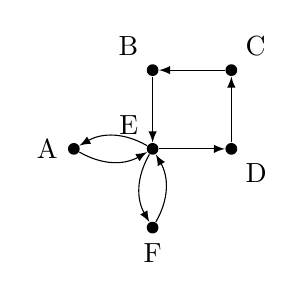
\begin{tikzpicture}[>=latex, scale=1,
	sommet/.style={fill, circle, inner sep=1.5}]
	\node[sommet, label=west:{A}] (A) at (1,2) {};
	\node[sommet, label=north west:{E}] (E) at (2,2) {};
	\node[sommet, label=south east:{D}] (D) at (3,2) {};
	\node[sommet, label=north east:{C}] (C) at (3,3) {};
	\node[sommet, label=north west:{B}] (B) at (2,3) {};
	\node[sommet, label=south:{F}] (F) at (2,1) {};
	
	\path (A) edge[->, bend right] (E);
	\path (E) edge[->, bend right] (F);
	\path (F) edge[->, bend right] (E);
	\path (E) edge[->] (D);
	\path (D) edge[->] (C);
	\path (C) edge[->] (B);
	\path (B) edge[->] (E);
	\path (E) edge[->, bend right] (A);
	
\end{tikzpicture}
\caption{}
\end{subfigure}
\begin{subfigure}[b]{.3\linewidth}
\centering
\shorthandoff{:}
\def\centerarc[#1](#2)(#3:#4:#5){ \draw[#1] ($(#2)+({#5*cos(#3)},{#5*sin(#3)})$) arc (#3:#4:#5); }
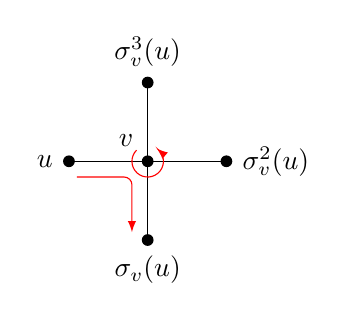
\begin{tikzpicture}[>=latex, scale=1, auto, swap,
	s/.style={fill, circle, inner sep=1.5}]
	\draw (0,1) node[s, label=left:{$u$}]{} -- (1,1) node[s, label=above left:{$v$}]{}-- (2,1) node[s, label=right:{$\sigma^2_v(u)$}]{};
	\draw (1,0) node[s, label=below:{$\sigma_v(u)$}]{} -- (1,2) node[s, label=above:{$\sigma^3_v(u)$}]{};
	\draw[red, rounded corners=2.8pt, ->] (0.1, 0.8) -- (0.8, 0.8) -- (0.8, 0.1);
	\draw[red,domain=135:415, xshift=1cm, yshift=1cm, ->] plot ({0.2*cos(\x)}, {0.2*sin(\x)});\end{tikzpicture}
\caption{}\label{sigma-u-v}
\end{subfigure}
\begin{subfigure}[b]{.3\linewidth}
\centering
\shorthandoff{:}
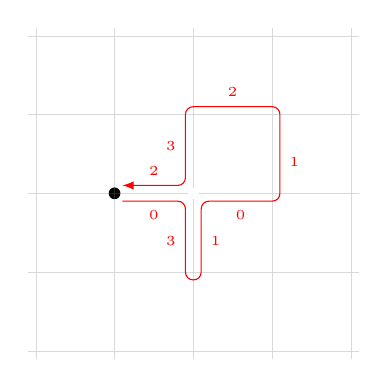
\begin{tikzpicture}[>=latex, scale=1, auto, swap]
	\node[fill, circle, inner sep=1.5] at (1,2) {};
	\draw[help lines, opacity=0.3] (-0.1,-0.1) grid (4.1, 4.1);
	\simplepath[->, very thick]{(2,2)}{02466};
	\node[fill=white, inner sep=0.2em] at (2,2) {};
	\simplepath[very thick]{(1,2)}{00};
	\draw[red, rounded corners=2.8pt, ->]  (1.1, 1.9) -- node{\tiny $0$} (1.9, 1.9) -- node{\tiny $3$} (1.9, 0.9) -- (2.1, 0.9) -- node{\tiny $1$} (2.1, 1.9) -- node{\tiny $0$} (3.1, 1.9) -- node{\tiny $1$} (3.1, 2.9) -- (3.1, 3.1) -- node{\tiny $2$} (1.9, 3.1) -- node{\tiny $3$} (1.9, 2.1) -- node{\tiny $2$} (1.1, 2.1);
\end{tikzpicture}
\caption{}
\end{subfigure}
\caption{Orientation du parcours de $\mathcal{G}(w)$}\label{fig:sequence-arcs}
\end{figure}

La justesse de la méthode découle de la «~règle de la main droite~» ou de «~l'algorithme du mur~» pour traverser un labyrinthe. En effet, étant donné l'arc $(u,v)$, prendre l'arc adjacent $(v,\sigma_v(u))$ revient à «~tourner à droite~» au sommet $v$ (voir figure \ref{sigma-u-v}). Le principe sous-jacent étant donc de commencer sur un point de l'enveloppe externe et rester dessus lors du parcours en prenant systématiquement à droite à chaque intersection, en terminant lors du retour au point de départ. Ceci garantit que le parcours est précisément l'enveloppe externe de $w$.

Pour implémenter efficacement cette méthode, plusieurs problèmes doivent être résolus. Premièrement, tel qu'indiqué plus haut, le parcours doit commencer sur un point de l'enveloppe externe sinon le résultat pourrait ne pas décrire l'objet voulu. On choisit donc le point $W$ associé au mot de contour $w$ comme point de départ.

Deuxièmement, lorsqu'un parcours repasse par $W$ on soit s'assurer que l'algorithme ne termine pas prématurément (le cas le plus simple étant codé par $w=\ocr{021}$, voir la figure \ref{chemin-et-enveloppe-externe}). Une solution simple consiste à construire une liste des voisins de $W$ dans le chemin $P$, et de les retirer lorsqu'ils sont visités. Cette liste contient au plus deux éléments puisqu'aucun sommet de $P$ ne peut se trouver à gauche ou en bas de $W$.

Le dernier problème à résoudre est la détection des intersections. Nous présenterons trois solutions solutions possibles avec des caractéristiques différentes. On cherche une fonction $f(x,y)\rightarrow \{1,0\}$ qui nous indique si l'emplacement $(x,y)$ a déjà été visité.

Première approche, l'adressage direct. Pour conserver la trace d'un chemin de longueur $n$ dans $\Z^2$, on  alloue immédiatement la mémoire pour l'ensemble de positions possibles dans un bloc contigu. On peut ainsi directement calculer l'emplacement de n'importe quelle position visitée. Un tableau $2n \times 2n$ contiendra toutes les positions atteignables par un chemin de longeur $n$ enraciné en $(n,n)$. Dans une telle structure de données, l'accès à une position spécifique se fait en temps constant. Par contre les besoins en mémoire sont  de l'ordre de $\O(n^2)$.

Deuxième approche, le tri. On ajoute chaque nouvelle position visitée à une liste triée. Plusieurs structures de données classiques se prêtent bien à cet usage comme les arbres rouge noir, les arbres B et les arbres AVL par exemple. Pour toutes ces structures de données bien connues, la consommation de mémoire est d'ordre $\O(n)$ et une opération de recherche ou d'insertion est d'ordre $\O(\log(n))$.

\newcommand{\voisin}{\text{\scshape voisin}\xspace}
\newcommand{\enfant}{\text{\scshape enfant}\xspace}
\newcommand{\pere}{\text{\scshape pere}\xspace}
\newcommand{\parcours}{\text{\scshape parcours}\xspace}
\newcommand{\HULL}{\text{\scshape hull}\xspace}

\newcommand{\Nodes}{\mathcal{N}}
\newcommand{\Node}[1]{\fbox{\vphantom{(}#1}}


Troisième approche, l'arbre radix augmenté \cite{BKP}. Soit $G=(\Nodes,E,V)$ un graphe où :
\setlist[description]{font=\normalfont}
\begin{description}
\item[$\Nodes$] Les sommets du graphe, on dira les noeuds, associés aux points de $\Z^2$.
\item[E] Les arêtes du graphe associées à la fonction \enfant.
\item[V] Les arêtes du graphe associées à la fonction \voisin.
\end{description}
On profite du fait que chaque accès est adjacent au précédent. Un noeud $N\in \mathcal{N}$ est défini par le quintuplet $N=(C, E, V, P, \Sigma)$ où $C\in \Z^2$ est la coordonnée cartésienne de ce noeud, $E=(E_0, E_1, E_2, E_3)$ où $E_i\in \mathcal{N}$ sont les quatre enfants, $V=(V_0,V_1,V_2,V_3)$ où $V_i\in{\mathcal{N}}$ sont les voisins, $P\in{\mathcal{N}}$ est le père et $\Sigma\in{\N}$ un compteur du nombre de fois où $N$ est visité. De plus, on permettra d'étiqueter les $V_i$ pour reconnaître un voisin \emph{explicite}, spécifié par le chemin parcouru, ou \emph{implicite}, ajouté par l'algorithme pour accélérer les calculs.

On notera le noeud du point $p$ à l'aide d'une boîte \Node{$p$} et on utilisera la forme \Node{$(x,y)$} pour le noeud de coordonnée $(x,y)$. 

Tout d'abord on considère un arbre contenant les points du plan, construit d'après la fonction $e:\Nodes \rightarrow \Nodes^4$ qui permet de passer d'un noeud à ses 4 enfants:
\begin{equation}
e\left(\Node{$(x,y)$}\right) = \left ( \Node{$(2x,2y)$},\Node{$(2x+1,2y)$},\Node{$(2x+1,2y+1)$},\Node{$(2x,2y+1)$}\right )\text{.}
\end{equation}

On définit la fonction $\text{\scshape enfant}$ comme une restriction de $e$ à l'enfant auquel on souhaite accéder : $$\text{\scshape enfant} : \Nodes \times \Z^2 \rightarrow \Nodes $$ où $\text{\scshape enfant}\left(\Node{$A$}, (x,y)\right) = \Node{$(x,y)$}$ est définie si et seulement si $\Node{$(x,y)$}$ est bel et bien un enfant de $\Node{$A$}$.

On remarque que les coordonnées des enfants sont obtenues en ajoutant $1$ ou $0$ à la représentation binaire des coordonnées du parent tel qu'illustré à la figure \ref{fig:arbre-radix-binaire}.

\begin{figure}
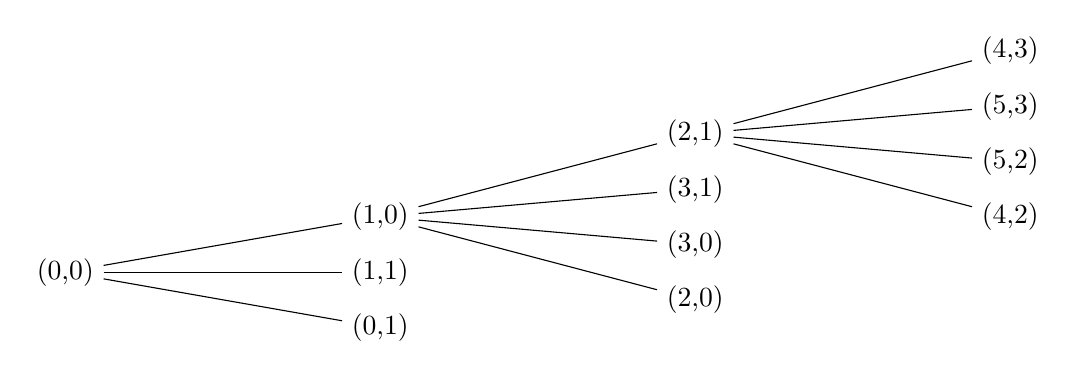
\begin{tikzpicture}[grow=right, sibling distance=2em,
					level distance=4cm]]

\node{(0,0)} 
	child {node {(0,1)}
	}
	child {node {(1,1)}
	}
	child {node {(1,0)}
		child {node {(2,0)}
		}
		child {node {(3,0)}
		}
		child {node {(3,1)}
		}
		child {node {(2,1)}
			child {node {(4,2)}}
			child {node {(5,2)}}
			child {node {(5,3)}}
			child {node {(4,3)}}
		}
	}
;
\end{tikzpicture}

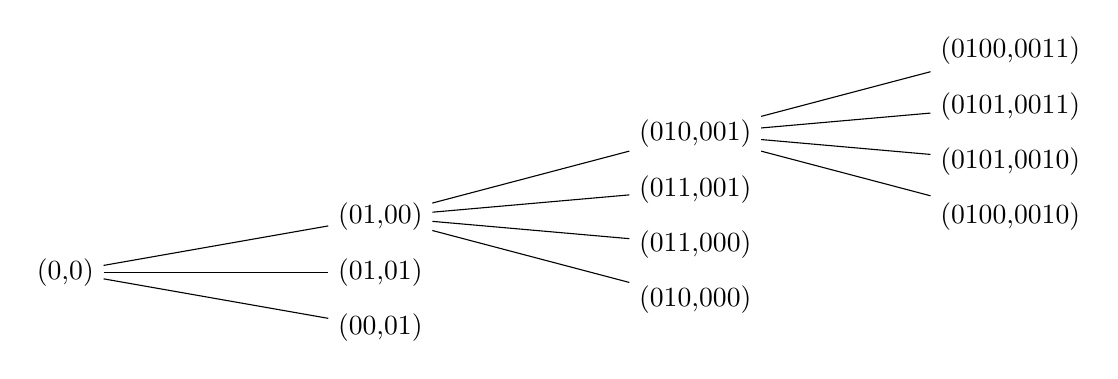
\begin{tikzpicture}[grow=right, sibling distance=2em,
					level distance=4cm]]

\node{(0,0)} 
	child {node {(00,01)}
	}
	child {node {(01,01)}
	}
	child {node {(01,00)}
		child {node {(010,000)}
		}
		child {node {(011,000)}
		}
		child {node {(011,001)}
		}
		child {node {(010,001)}
			child {node {(0100,0010)}}
			child {node {(0101,0010)}}
			child {node {(0101,0011)}}
			child {node {(0100,0011)}}
		}
	}
;
\end{tikzpicture}
\caption{Arbre radix et sa représentation binaire.}\label{fig:arbre-radix-binaire}
\end{figure}

La fonction inverse $$\pere: \Nodes \rightarrow \Nodes$$ permet de passer d'un noeud à son père. On peut aussi calculer directement les coordonnées du père:
\begin{equation}
f(x,y) = \left(\floor*{\frac{x}{2}}, \floor*{\frac{y}{2}}\right)
\end{equation} 
Le fait de connaître les coordonnées du père d'un point sans avoir de référence au noeud de ce point ou à celui de son père est crucial au fonctionnement de l'algorithme. 

\begin{figure}
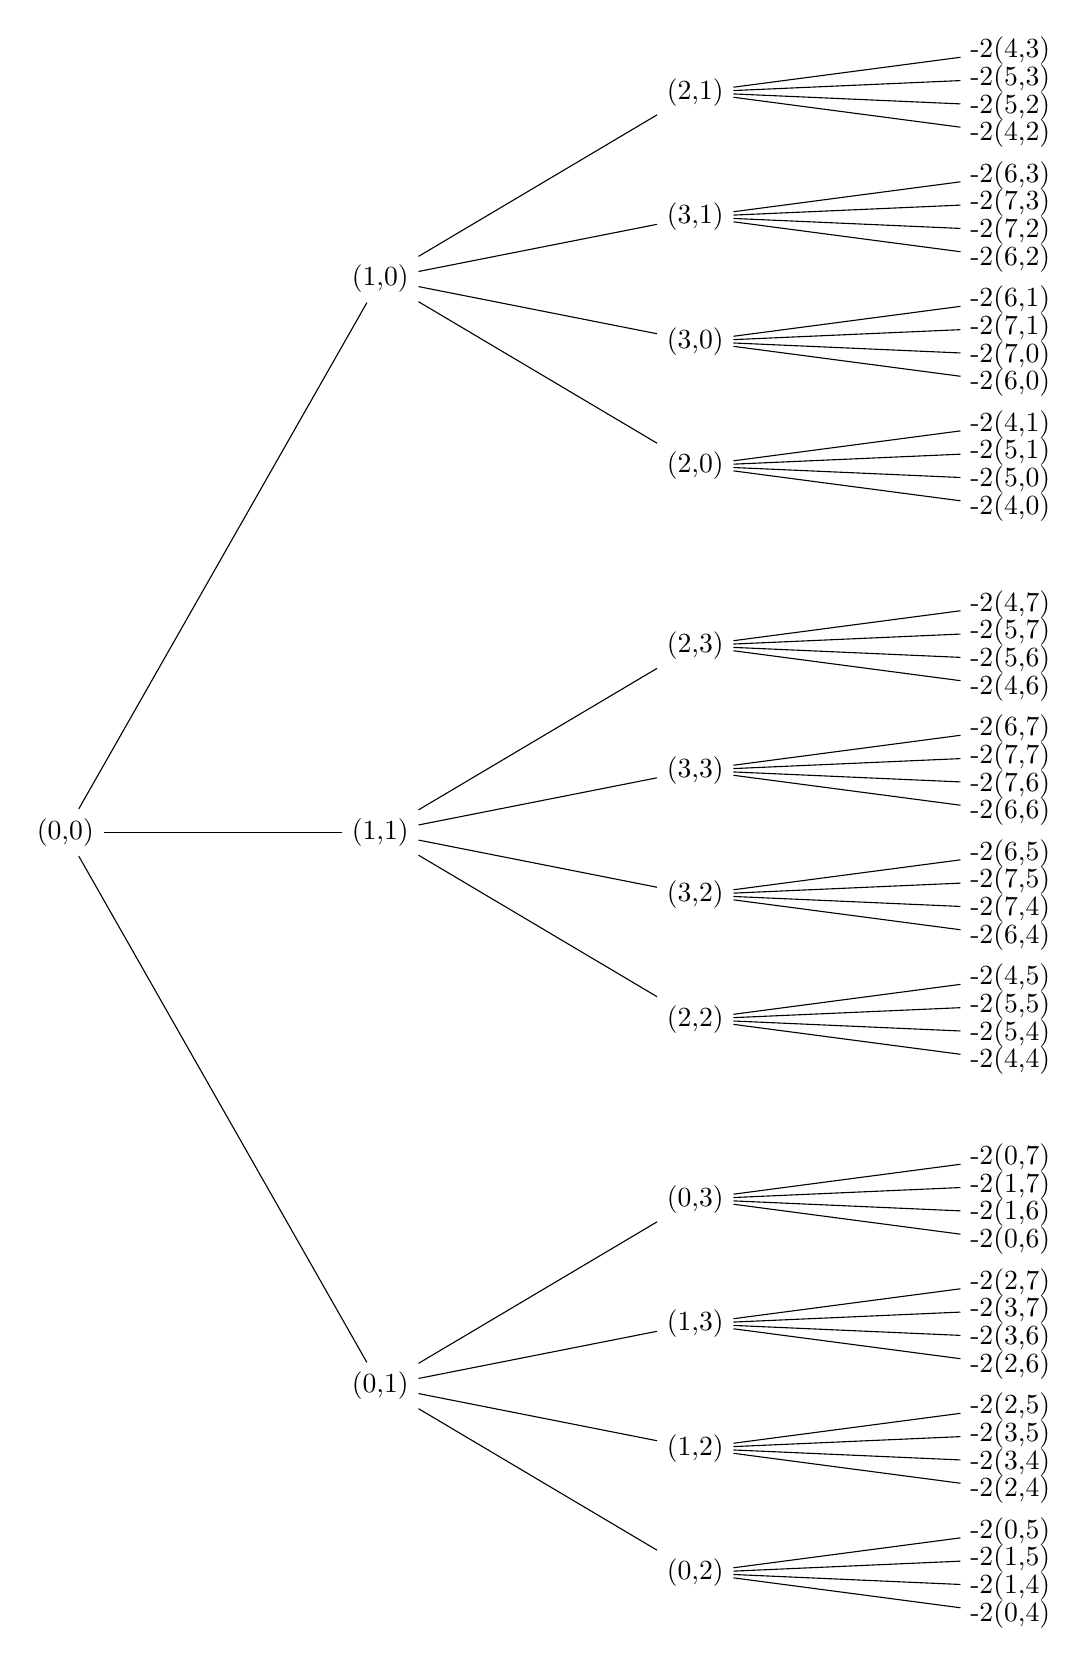
\begin{tikzpicture}[grow=right, 
					level 1/.style={sibling distance=20em},
					level 2/.style={sibling distance=4.5em},
					level 3/.style={sibling distance=1em, font=\relsize{-2}}, 
					level distance=4cm]]

\node{(0,0)} 
	child {node {(0,1)}
		child {node {(0,2)}
			child {node {(0,4)}}
			child {node {(1,4)}}
			child {node {(1,5)}}
			child {node {(0,5)}}
		}
		child {node {(1,2)}
			child {node {(2,4)}}
			child {node {(3,4)}}
			child {node {(3,5)}}
			child {node {(2,5)}}
		}
		child {node {(1,3)}
			child {node {(2,6)}}
			child {node {(3,6)}}
			child {node {(3,7)}}
			child {node {(2,7)}}
		}
		child {node {(0,3)}
			child {node {(0,6)}}
			child {node {(1,6)}}
			child {node {(1,7)}}
			child {node {(0,7)}}
		}
	}
	child {node {(1,1)}
		child {node {(2,2)}
			child {node {(4,4)}}
			child {node {(5,4)}}
			child {node {(5,5)}}
			child {node {(4,5)}}
		}
		child {node {(3,2)}
			child {node {(6,4)}}
			child {node {(7,4)}}
			child {node {(7,5)}}
			child {node {(6,5)}}
		}
		child {node {(3,3)}
			child {node {(6,6)}}
			child {node {(7,6)}}
			child {node {(7,7)}}
			child {node {(6,7)}}
		}
		child {node {(2,3)}
			child {node {(4,6)}}
			child {node {(5,6)}}
			child {node {(5,7)}}
			child {node {(4,7)}}
		}
	}
	child {node {(1,0)}
		child {node {(2,0)}
			child {node {(4,0)}}
			child {node {(5,0)}}
			child {node {(5,1)}}
			child {node {(4,1)}}
		}
		child {node {(3,0)}
			child {node {(6,0)}}
			child {node {(7,0)}}
			child {node {(7,1)}}
			child {node {(6,1)}}
		}
		child {node {(3,1)}
			child {node {(6,2)}}
			child {node {(7,2)}}
			child {node {(7,3)}}
			child {node {(6,3)}}
		}
		child {node {(2,1)}
			child {node {(4,2)}}
			child {node {(5,2)}}
			child {node {(5,3)}}
			child {node {(4,3)}}
		}
	}
;
\end{tikzpicture}
\caption{Les 4 premiers niveaux de l'arbre radix de $\N^2$.}
\end{figure}

L'arbre est initialisé à une certaine position avec ses liens pères jusqu'à la racine en \Node{$(0,0)$}. La racine est son propre père. La figure \ref{radix-tree-N} illustre de quelle façon on divise le plan entre les différents niveaux de l'arbre.

La seule façon d'obtenir une référence à un nouveau noeud est par la fonction {\scshape enfant}, $f$ ne fait que calculer les coordonnées.

\newcommand{\surround}[2]{\draw[rounded corners] ($#2-(1em,1em)$) rectangle ($#2 + (#1,#1) + (1em,1em)$);}
\newcommand{\drawpointgrid}{
\foreach \x in {0,1,...,15}
  \foreach \y in {0,1,...,15}
  {
  \node[draw, circle, inner sep=0.05em, fill] at (\x,\y) {};
  }

\draw[rounded corners] ($(0,1) + (-1em,-1em)$) -- ($(0,1) + (-1em,1em)$) --
				       ($(1,1) + (1em,1em)$) -- ($(1,0) + (1em,-1em)$) --
				       ($(1,0) + (-1em,-1em)$) -- ($(1,1) + (-1em,-1em)$) -- cycle;


\draw[rounded corners] ($(0,2) + (-1em,-1em)$) -- ($(0,3) + (-1em,1em)$) --
				       ($(3,3) + (1em,1em)$) -- ($(3,0) + (1em,-1em)$) --
				       ($(2,0) + (-1em,-1em)$) -- ($(2,2) + (-1em,-1em)$) -- cycle;


\draw[rounded corners] ($(0,4) + (-1em,-1em)$) -- ($(0,7) + (-1em,1em)$) --
				       ($(7,7) + (1em,1em)$) -- ($(7,0) + (1em,-1em)$) --
				       ($(4,0) + (-1em,-1em)$) -- ($(4,4) + (-1em,-1em)$) -- cycle;

\draw[rounded corners] ($(0,8) + (-1em,-1em)$) -- ($(0,15) + (-1em,1em)$) --
				       ($(15,15) + (1em,1em)$) -- ($(15,0) + (1em,-1em)$) --
				       ($(8,0) + (-1em,-1em)$) -- ($(8,8) + (-1em,-1em)$) -- cycle;



}

\newenvironment{pointgrid}
{
\begin{tikzpicture}[auto, >=latex, shorten >=.2em, scale=.83]
\drawpointgrid
}
{
\end{tikzpicture}
}



\begin{figure}
\begin{pointgrid}
\node[label={[label distance=-.5em]\tiny (0,0)}] at (0,0) {} edge[bend right, ->] (1,0) edge[->, loop below] (0,0);
\node[label={[label distance=-.5em]\tiny (1,0)}] at (1,0) {} edge[bend right, ->] (3,1);
\node[label={[label distance=-.5em]\tiny (3,1)}] at (3,1) {} edge[bend right, ->] (7,2);
\node[label={[label distance=-.5em]\tiny (7,2)}] at (7,2) {} edge[bend right, ->] (15,4);
\node[draw, circle, inner sep=0.15em, label={[label distance=-.3em]\tiny (15,4)}] at (15,4) {};

\node at (-2,0) {Niveau 0};
\node at (-2,1) {Niveau 1};
\node at (-2,2.5) {Niveau 2};
\node at (-2,5.5) {Niveau 3};
\node at (-2,11.5) {Niveau 4};
\end{pointgrid}

\caption{Cinq premiers niveaux de l'arbre radix de $\N^2$ initialisé en $(15,4)$.}\label{radix-tree-N}
\end{figure}

Le lemme suivant stipule que des noeuds voisins ont le même père ou leurs pères sont voisins.

\begin{lemma}\label{lemme-parents-voisins}
Soit $a$,$b$ $\in \Z^2$ et $\Delta\in \{{(1,0),(0,1),(−1,0),(0,−1)}\}$ tel que $a+\Delta=b$, alors l'une des deux conditions suivantes est vraie : 
\begin{enumerate}
\item $f(a) = f(b)$
\item $f(a)+\Delta = f(b)$.
\end{enumerate}

\end{lemma}
\begin{proof}
Puisque $a$ et $b$ sont voisins, on suppose sans perdre de généralité que $\Delta \in \{(-1,0),(1,0)\}$ donc $b_x=a_x + \Delta_x$ et $a_y=b_y$. On pose $x = f(a)_x$ alors par définition $a_x$ est de forme $2x$ ou $2x+1$. Le tableau \ref{voisinage-parents} récapitule les quatre cas possibles. On constate qu'on a bien $f(a)_x = f(b)_x$ ou $f(a)_x+\Delta_x = f(b)_x$ dans chacun des cas, tel que voulu.

\begin{table}
\centering
\begin{tabular}{|c|c|c|c|c|c|}
\hline
$a_x$ & $\Delta_x$ & $b_x$ & $f(a)_x$ & $f(b)_x$ & $f(a)_x+\Delta_x$ \\
\hline
$2x$ & $1$ & $2x + 1$ & $x$ & $x$ & $x+1$ \\
$2x$ & $-1$ & $2x - 1$ & $x$ & $x-1$ & $x-1$ \\
$2x+1$ & $1$ & $2x+1 + 1$ & $x$ & $x+1$ & $x+1$ \\
$2x+1$ & $-1$ & $2x+1 - 1$ & $x$ & $x$ & $x-1$ \\
\hline
\end{tabular}
\caption{Voisinage des parents lorsque $a$ et $b$ sont voisins.}\label{voisinage-parents}
\end{table}

\end{proof}

L'algorithme \voisin obtient une référence au voisin d'un noeud à l'aide d'un appel récursif à son père en vertu du lemme \ref{lemme-parents-voisins}:
$$\voisin : \Nodes \times \Z^2 \rightarrow \Nodes\text{.}$$

Soit $\Node{a}=(C, E, V, P, \Sigma)\in \Nodes$ et $\Node{b}\in \Nodes$ des noeuds. 
On introduit la notation $\Node{$a$} \stackrel{\Delta}{\rightarrow} \Node{$b$}$ où $\Delta \in \F$, qui représente 
le voisin $V_\Delta$ du noeud $\Node{$a$}$. Puisque notre structure de donnée est allouée 
dynamiquement, le voisin de $\Node{$a$}$ en direction $\Delta$ 
n'est pas encore connu lors du premier appel $\voisin\left(\Node{$a$}, \Delta\right)$. 
On initialise $\Node{$a$} \stackrel{\Delta}{\rightarrow} \Node{$b$}$ avec $\Node{$a$}_{V_\Delta} = \Node{$b$}$.

% on redéfinit FUNCTION pour avoir des parenthèses dynamiques. 
% ATTENTION -- on brise les paramètres vides.
\algdef{SE}[FUNCTION]{Function}{EndFunction}%
   [2]{\algorithmicfunction\ \textproc{#1}$\left(\text{#2}\right)$}%
   {\algorithmicend\ \algorithmicfunction}%
   
\begin{algorithm}
	\fontsize{10}{10}\selectfont
	\begin{algorithmic}[1]
	\Require $\Node{$o$} \in \Nodes$, $\Delta \in \F$
	\Ensure $\Node{$o$} \stackrel{\Delta}{\rightarrow} \Node{$d$}$ correctement initialisé
	\Function{voisin}{\Node{$o$}, $\Delta$}
		\If{ $\Node{$o$} \stackrel{\Delta}{\rightarrow} \Node{$d$}$ n'est pas initialisé}
			\State $p \gets \text{Pas élémentaire associé à } \Delta$
			\State $d \gets o + p$
			\If{$d$ est un fils de $o$}
				\State $\Node{$d$} \gets \enfant \left(\Node{$o$}, d \right)$
			\Else
			\State $\Node{pere} \gets \pere \left(\Node{$o$}\right)$
			\If{$f(d) = pere$}
				\State $\Node{$d$} \gets \enfant \left(\Node{pere}, d\right)$
			\Else													
				\State $\Node{$d$} \gets \enfant \left(\voisin \left(\Node{pere}, \Delta\right), d\right)$
			\EndIf
			\EndIf
			\State initialiser $\Node{$o$} \stackrel{\Delta}{\rightarrow} \Node{$d$}$
			\State initialiser $\Node{$d$} \stackrel{\bar{\Delta}}{\rightarrow} \Node{$o$}$
		\EndIf
		\State \Return $\Node{$d$}$
	\EndFunction
	\end{algorithmic}
\caption{\voisin}\label{algorithme-parcours}
\end{algorithm}

On obtient ensuite naturellement l'algorithme \parcours en invoquant \voisin avec chaque lettre du mot $w$.
$$\parcours : \F^* \times \Nodes \rightarrow \Nodes$$

\begin{algorithm}
	\fontsize{10}{10}\selectfont
	\begin{algorithmic}[1]
	\Require $w \in \F^*$ où $|w|=n$, $\Node{o} \in \Nodes$ initialisé jusqu'à la racine.
	\Ensure $\Node{$r$}\in \Nodes$ le dernier noeud visité après la lecture de $w$.
	
	\Function{parcours}{$w$, \Node{$o$}}
		\State incrémenter $\Sigma$ de $\Node{$o$}$.
		\If{|w| = 0}
			\State $\Node{$r$} \gets \Node{$o$}$
		\Else
			\State $\Node{$d$} \gets \voisin\left(\Node{$o$}, \Delta \right)$
			\State étiqueter explicite le lien de voisinage $V_\Delta$ de \Node{$o$}
			\State étiqueter explicite le lien de voisinage $V_{\bar\Delta}$ de \Node{$d$}
			\State $\Node{$r$} \gets \parcours\left( w_{1..n}, \Node{$d$} \right)$
		\EndIf
		\State \Return $\Node{$r$}$
	\EndFunction
	\end{algorithmic}
\caption{\parcours}\label{algorithme-voisin}
\end{algorithm}




La séquence qui suit illustre la progression de l'algorithme \parcours lors de la lecture du mot \ocr{222} à partir du point $(15,4)$.
\begin{enumerate}
\foreach \n in {1,...,12}{\item \adjustbox{valign=t}{\includegraphics[page=\n,scale=.9]{figures/radix-tree-trace.pdf}} }
\end{enumerate}

Voyons maintenant comment étendre cette structure aux autres quadrants du plan. L'astuce consiste à remplacer la racine de l'arbre par un noeud virtuel, $\alpha$ qui n'appartient pas à $\Z^2$ mais a quatre enfants, un dans chaque quadrant, 
\begin{equation}
e\left(\Node{$\alpha$}\right)=\left(\Node{$(0,0)$}, \Node{$(0,-1)$}, \Node{$(-1,-1)$}, \Node{$(-1,0)$}\right)
\end{equation}
Pour détecter un enfant de $\alpha$, on utilise la propriété $f(d)=d$, vraie si et seulement si $d$ est un enfant de $\alpha$. Il suffit ensuite de faire une légère modification à l'algorithme \voisin tel qu'indiqué en rouge dans l'algorithme \ref{algorithme-voisin-plan}. On note que les coordonnées, les voisins et le père de $\alpha$ sont indéfinis, mais que l'algorithme n'y accède jamais.

\begin{algorithm}
	\fontsize{10}{10}\selectfont
	\begin{algorithmic}[1]
	\Require $\Node{$o$} \in \Nodes$, $\Delta \in \F$
	\Ensure $\Node{$o$} \stackrel{\Delta}{\rightarrow} \Node{d}$ correctement initialisé
	\Function{voisin}{\Node{$o$}, $\Delta$}
		\If{ $\Node{$o$} \stackrel{\Delta}{\rightarrow} \Node{d}$ n'est pas initialisé}
			\State $d \gets o + \Delta$
			\If{$d$ est un fils de $o$}
				\State $\Node{$d$} \gets \enfant \left(\Node{$o$}, d \right)$
			\Else
			\State $\Node{pere} \gets \text{\scshape pere}\left(\Node{$o$}\right)$
			\If{${\color{red}f(d) = d}$ ou $f(d) = pere$}										
				\State $\Node{$d$} \gets \text{\scshape enfant}\left(\Node{pere}, d\right)$
			\Else													
				\State $\Node{$d$} \gets \text{\scshape enfant}\left(\text{\scshape voisin}\left(\Node{pere}, \Delta\right), d\right)$
			\EndIf
			\EndIf
			\State initialiser $\Node{$o$} \stackrel{\Delta}{\rightarrow} \Node{$d$}$
			\State initialiser $\Node{$d$} \stackrel{\bar{\Delta}}{\rightarrow} \Node{$o$}$
		\EndIf
		\State \Return $\Node{$d$}$
	\EndFunction
	\end{algorithmic}
\caption{\voisin étendu au plan}\label{algorithme-voisin-plan}
\end{algorithm}

\begin{figure}
\foreach \n in {1,...,12}{\begin{subfigure}[b]{.3\textwidth}\centering\includegraphics[page=\n, scale=1.1]{figures/radix-tree-trace-quadrant.pdf}\subcaption{}\end{subfigure}
}
\caption{Changement de quadrant}
\end{figure}

Avant d'aborder le théorème de linéarité de \parcours, on remarquera d'abord qu'on peut compter les ancêtres de $\Node{n} \in \Nodes$ grâce à la fonction $f$
\begin{equation}
\left|\bigcup_{i=1}^h \pere^i\left(\Node{n}\right)\right| = \left|\bigcup_{i=1}^{h}f^i(n)\right| + 1
\end{equation}
ainsi on pourra effectuer les démonstrations dans $\Z^2$ plutôt que dans $\Nodes$. De plus, il sera utile d'étendre $f$ aux ensembles de points et finalement, nous aurons besoins du lemme suivant pour borner le nombre de noeuds créés.

\begin{figure}
\centering
\includegraphics{figures/etendu-au-plan.pdf}\caption{Les points du plan regroupés par parent}
\end{figure}

\begin{lemma}\label{lemme-moins-de-peres}
Soit $E=\left\{p_0, p_1, p_2, p_3, p_4\right\}$ où $p_i \in \Z^2$ et $w \in \F^4$ tel que pour $i=0,1,2,3$ on a $p_{i+1} = p_{i} + w_i$, alors $\left|f(E)\right| \leq 4$.
\end{lemma}
\begin{proof}
L'arbre radix divise le plan en sections de $2\times2$ points partageant le même père. Par conséquent, au moins deux $p_i$ partagent le même père, d'où la borne $|f(E)| \leq 4$.
\end{proof}

\begin{theorem}\emph{\cite{BKP}.}
L'algorithme \parcours est linéaire.
\end{theorem}

\begin{proof}
On remarque d'abord que l'essentiel du temps passé dans \voisin est causé par l'appel récursif, puisque toutes les autres opérations sont d'ordre constant. Donc $\voisin$ est d'ordre $\O($h$)$ où $h$ est la hauteur de l'arbre. Cependant, un appel récursif n'est effectué sur un noeud que la première fois où l'un de ses enfants recherche son voisin, le résultat étant stocké directement au niveau de l'enfant la suite. Ainsi, pour tout noeud, \voisin est appelé un maximum de 16 fois (les quatre voisins de ses quatre enfants). Le temps total passé dans \voisin est donc proportionnel au nombre de noeuds créés. Reste à montrer que \parcours créé un nombre de noeuds proportionnel à $|w|$.

Soit $N$ tous les noeuds créés et $N_v \subseteq N$ les noeuds visités. On va montrer que le nombre total de noeuds créés est borné par un multiple du nombre de noeuds visités. Clairement, $|N_v| ≤ |N|$ et $|N_v| ≤ |w|$. De plus, on obtient $N$ à partir de $N_v$ grâce à $f$, $N = \bigcup_{i=0}^{h}f^i(N_v)$ donc
\begin{equation}\label{eq:nv-n}
|N| = \sum_{i=0}^{h} \left| f^i(N_v) \right|\text{.}
\end{equation}

Par construction chaque noeud ajouté à $N_v$ est voisin de son précédent. Le lemme \ref{lemme-moins-de-peres} s'applique et on regroupe les éléments par 5
\begin{equation}\label{eq:4-5emeNv}
|f(N_v)| ≤ 4 \left \lceil \frac{|N_v|}{5} \right \rceil ≤ \frac{4}{5}(|N_v| + 4)
\end{equation}

Le lemme \ref{lemme-parents-voisins} nous permet d'appliquer récursivement le lemme \ref{lemme-moins-de-peres} sur $f$. On combine donc les équations \ref{eq:nv-n} et \ref{eq:4-5emeNv} pour obtenir l'expression
\begin{equation}
|N| ≤ \sum_{i=0}^{h} \left| f^i(N_v) \right| ≤ \sum_{i=0}^{h} \left( \left( \frac{4}{5} \right)^i |N_v| + \sum_{j=0}^{i} \left( \frac{4}{5} \right)^j 4 \right) ≤ \cdots
\end{equation}
qu'on borne ensuite à l'aide de l'identité $\sum_{i=1}^\infty \left(\frac{4}{5}\right)^i=5$ pour finalement avoir
\begin{equation}
\cdots ≤ 5|N_v| + 4 \sum_{i=0}^{h} 5 ≤ 5|N_v| + 20h
\end{equation}

Puisque $h$ est précisément le nombre de bits requis pour écrire les coordonnées des points dans $N$, $h\in \O(\log n)$ et ainsi $|N| \in \O(n)$. Finalement, puisque $N_v ≤ |w|$ on a que $\parcours \in \O(|w|)$, tel que voulu.
\end{proof}

Le tableau \ref{fig:recapitulation-intersections} récapitule les avantages et les désavantages des trois méthodes de détection d'intersection présentées pour un chemin $w$ de longueur $|w|=n$

\begin{table}
\begin{tabular}{|l|l|l|l|}
\hline
Méthode & Complexité & Commentaires \\
\hline
Adressage direct & $\O(n^2)$ & \parbox{.6\textwidth}{\vspace{.33\baselineskip}
\begin{itemize}[leftmargin=*]
\item Rapide pour les petites valeurs de $n$.
\item Structure de données native en informatique.
\item On doit connaître $n$ au départ.
\end{itemize}\vspace{.25\baselineskip}}\\
\hline
Tri & $\O(n \log n)$ & \parbox{.6\textwidth}{\vspace{.33\baselineskip}
\begin{itemize}[leftmargin=*]
\item Méthode la moins gourmande en mémoire.
\item On n'a pas à connaître $n$ au départ.
\item Structures de données déjà implémentées sous forme de librairies.
\end{itemize}\vspace{.25\baselineskip}}\\
\hline
BKP & $\O(n)$ & \parbox{.6\textwidth}{\vspace{.33\baselineskip}
\begin{itemize}[leftmargin=*]
\item On n'a pas à connaître $n$ au départ.
\item Maintient sa performance même avec les chemins très longs.
\item Plus lent que les autres méthodes pour les chemins courts.
\end{itemize}\vspace{.25\baselineskip}}\\
\hline
\end{tabular}
\caption{Récapitulation des méthodes de détection d'intersection}\label{fig:recapitulation-intersections}
\end{table}

On en arrive à l'algorithme principal de ce chapitre.

\begin{algorithm}
	\fontsize{10}{10}\selectfont
	\begin{algorithmic}[1]
	\Require Un mot $w \in \F^*$ codant un chemin discret.
	\Ensure Un mot $w' \in F^*$ codant $\hull{w}$.
	\Function{hull}{$w$}
		\State Invoquer $\parcours$ sur le mot $w$ à partir de $(0,0)$. \label{initialisation}
		\State Soit $W$ un point de la factorisation standard. \label{c1a}
		\State Soit $V$ l'ensemble des voisins explicites de $W$. \label{c1b}
		\State $c \gets V_0$ \label{c1c}
		\State $w' = \text{Step}(c-W)$ \label{w'initialise} \label{c1d}
		\While {$c \neq W$ ou $|V| \neq 0$}\label{boucle}
			\State $turn \gets 2$
			\For{chaque voisin explicite $v$ de $c$}\label{pour-chaque-voisin}
				\State $\Delta \gets \text{Step}(v-c)$
				\If{$\left( \Delta - w'_{n-1} \right)+1 \mod 4 ≤ turn + 1 \mod 4$}
					\State $turn \gets \Delta - w'_{n-1}$
					\State $suivant \gets v$
				\EndIf
			\EndFor \label{pour-chaque-voisin-fin}
			\State $w' = w' \cdot \Delta$ \label{grow-w'}
			\State Retirer $c$ de $V$ \label{vider-grand-V}
			\State $c \gets suivant$
		\EndWhile
		\State \Return $w'$
	\EndFunction
	\end{algorithmic}
\caption{Algorithme \HULL}\label{algorithme-hull}
\end{algorithm}

On commence à la ligne \ref{initialisation} par construire l'arbre radix augmenté associé au mot $w$. En commençant au point $c=W$, on procède pour chaque position $c$
\begin{enumerate}
\item Extraire la lettre $\Delta\in\F$ associée au vecteur $\vec{cv}$ pour chaque voisin $v$ de $c$.
\item Déterminer le virage associé à chaque $\Delta$.
\item Choisir le virage le plus à droite, c'est à dire celui le plus proche de $3$.
\end{enumerate}
L'algorithme se termine lorsqu'on revient au point $W$.

\begin{theorem}[Justesse de l'algorithme \ref{algorithme-hull}.] Pour chaque mot $w\in\F^*$ l'algorithme \ref{algorithme-hull} calcule $\hull{w}$.
\end{theorem}

\begin{proof}
Soit $\hull{w}$ de longeur $k\in \N$. On utilise l'invariant de boucle suivant:

\blockquote{Au début de la $i$-ième itération de la boucle à la ligne \ref{boucle}, $w'$ est un préfixe de longeur $i$ du mot de contour associé à $\hull{w}$.}

L'invariant tient lors de la première itération de la boucle à la ligne \ref{boucle}, puisqu'à ce moment $w'$ a été initialisé à la ligne \ref{w'initialise}. On suppose donc que l'invariant tient encore au début de la $i$-ième itération. $w'$ est alors un préfixe de longeur $i$ de $\hull{w}$. Les lignes \ref{pour-chaque-voisin} à \ref{pour-chaque-voisin-fin} calculent la direction du voisin le plus à droite et la ligne \ref{grow-w'} concatène cette direction à $w'$. Par la règle de la main droite, choisir le voisin le plus à droite assure de demeurer sur l'enveloppe extérieure de $w$. Ainsi, à la fin de la $i$-ième itération, $w'$ est un préfixe du mot de contour associé à $\hull{w}$ de longueur $i+1$. Finalement, à la fin de la boucle, $w'$ est un préfixe de $\hull{w}$ de longueur $k$, autrement dit $w'=\hull{w}$. Notons que puisque tous les voisins de $W$ sont sur l'enveloppe externe, la ligne \ref{vider-grand-V} retire bien tous les éléments de $V$ ce qui garantit que l'algorithme se termine.
\end{proof}

Nous terminons maintenant cette section en démontrant que l'algorithme \ref{algorithme-hull} est linéaire en temps et en espace. On a déjà démontré que \parcours est linéaire en temps. On peut facilement obtenir $W$ lors du parcours initial sans aucun coût supplémentaire. Les lignes \ref{c1a}, \ref{c1b}, \ref{c1c} et \ref{c1d} s'exécutent toutes en temps constant. Ensuite, la boucle extérieure à la ligne \ref{boucle} est exécutée exactement $k$ fois, une fois pour chaque lettre de $w'$ et $|w'| ≤ |w|$. Pour chaque itération de la boucle extérieure, la boucle intérieure s'exécute un maximum de $4$ fois. Le temps total de la boucle est donc de $k(4 c_1 + c_2)$, où $c_1$ et $c_2$ sont des constantes appartenant à $\R$, ce qui montre bien que l'algorithme \ref{algorithme-hull} dans son ensemble est linéaire en temps. On termine la preuve en remarquant que l'arbre radix augmenté est linéaire en espace et qu'aucun nouveau noeud n'est créé après l'appel initial à \parcours.